% This file was created with tikzplotlib v0.10.1.
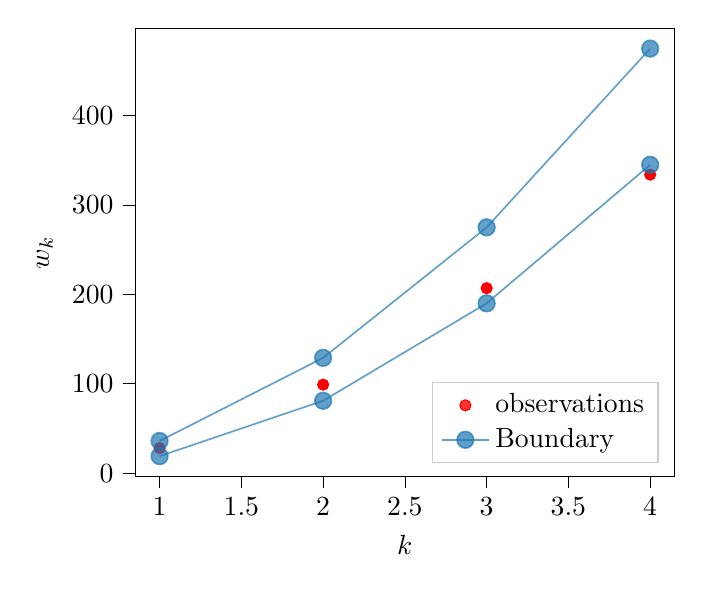
\begin{tikzpicture}

\definecolor{darkgray176}{RGB}{176,176,176}
\definecolor{lightgray204}{RGB}{204,204,204}
\definecolor{steelblue31119180}{RGB}{31,119,180}

\begin{axis}[
legend cell align={left},
legend style={
  fill opacity=0.8,
  draw opacity=1,
  text opacity=1,
  at={(0.97,0.03)},
  anchor=south east,
  draw=lightgray204
},
tick align=outside,
tick pos=left,
x grid style={darkgray176},
xlabel={\(\displaystyle k\)},
xmin=0.85, xmax=4.15,
xtick style={color=black},
y grid style={darkgray176},
ylabel={\(\displaystyle w_k\)},
ymin=-3.8, ymax=497.8,
ytick style={color=black}
]
\addplot [draw=red, fill=red, mark=*, only marks]
table{%
x  y
1 28
2 99
3 207
4 334
};
\addlegendentry{observations}
\addplot [semithick, steelblue31119180, opacity=0.7, mark=*, mark size=3, mark options={solid}]
table {%
1 19
2 81
3 190
4 345
};
\addlegendentry{Boundary}
\addplot [semithick, steelblue31119180, opacity=0.7, mark=*, mark size=3, mark options={solid}, forget plot]
table {%
1 36
2 129
3 275
4 475
};
\end{axis}

\end{tikzpicture}
